The results from running the Jacobi rotation algorithm will vary with how 
$n_{\mathrm{step}}$ and $\rho_{max}$ are chosen. First of all, it would be useful to find
out how large the matrix needs to be for the algorithm to produce the first few
eigenvalues with four leading digits. At that point, the precision is high
enough for our purposes. Second, we'd like to see how the precision in the
eigenvalues depend on the choice of $\rho_{max}$. 

By doing more of a guess than calculation, we set $\rho_{max} = 5$. The
algorithm is then used to find the eigenvalues of matrices with increasing
dimensions. The range for $n_{\mathrm{step}}$ is narrowed down to $n_{\mathrm{step}} \in 
[150,300]$ to see the relative difference more clearly. Figure \refig{nreldiff} shows 
the result. 
%
\begin{figure}[htpb]
\centering
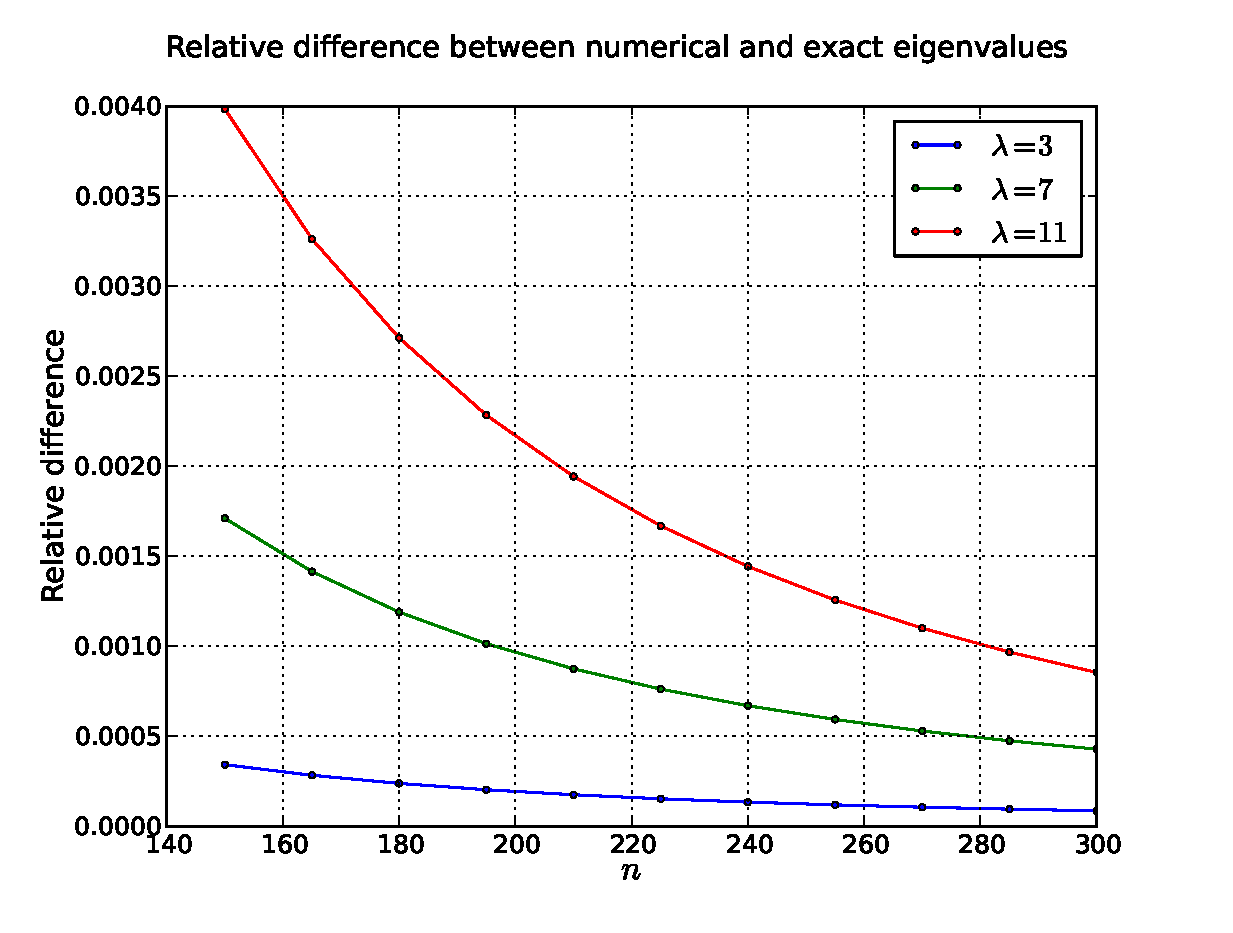
\includegraphics[width=1.0\textwidth]{images/nreldiff2.eps}
\caption{The figure shows how much the numerical eigenvalues differ from the analytical
	ones as $n_{\mathrm{step}}$ increases. Here we have $\rho_{max} = 5$.}
\label{fig:nreldiff}
\end{figure}
%
It's obvious that $\lambda_0 = 3$ varies the least, and has four correct leading digits
throughout the plot. The second eigenvalue $\lambda_1 = 7$ varies a bit more, and settles
at four correct leading digits for about $n_{\mathrm{step}} = 210$. The third eigenvalue,
$\lambda_2 = 11$, has four correct leading digits for all $n_{\mathrm{step}}$ that are shown in 
\refig{nreldiff}. This means that when $n_{\mathrm{step}} = 210$, all three eigenvalues show 
four correct leading digits. 

The precision of the eigenvalues will also depend on $\rho_{max}$. If we do the same
procedure as above, but keep $n_{\mathrm{step}}$ constant and vary $\rho_{max}$ instead, we get the
result shown in figure \refig{rhoreldiff}.
%
\begin{figure}[htpb]
	\centering
	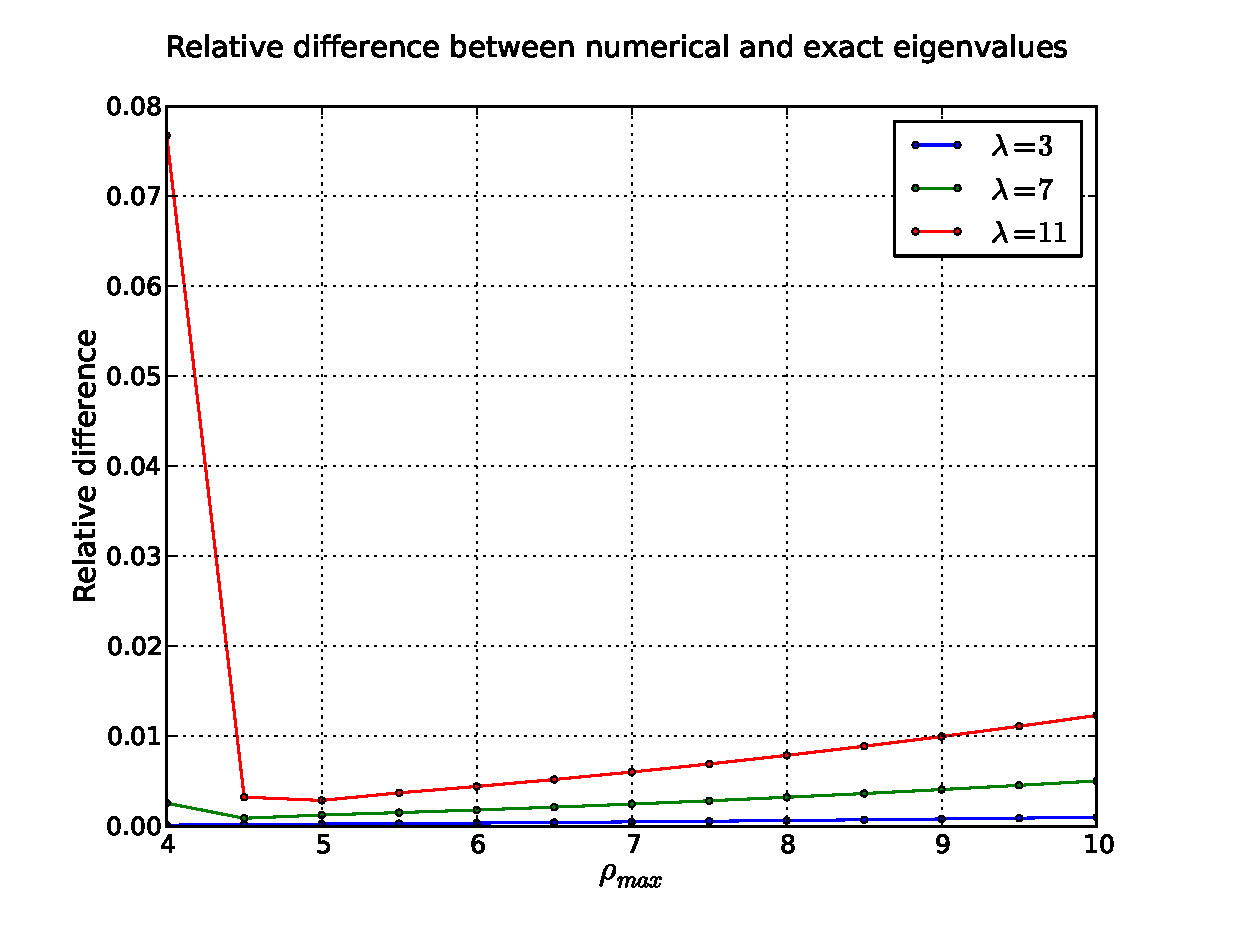
\includegraphics[width=1.0\textwidth]{images/reldiff2.eps}
	\caption{The figure shows how the numerical eigenvalues differ from the analytical
		ones as $\rho_{max}$ increases. Here we have $n_{\mathrm{step}} = 210$.}
	\label{fig:rhoreldiff}
\end{figure}
%
Again, the range of $\rho_{max}$ is narrowed down to $\rho_{max} \in [4,10]$ in order to
highlight the interesting part. For $\rho_{max} = 4$ both $\lambda_1$ and $\lambda_2$ are
below the precision we want. Already at the next step, $\rho_{max} = 4.5$, they both
reach four leading digit precision. This holds true for $\rho_{max} = 5$ as well, although
the graph grows a little. For higher values, the precision just lowers.
So far, we can conclude that $\rho_{max} = 4.5$ gives greatest accuracy.

It can be useful to know how many transformations are needed before all non-diagonal
elements have become zero. Of course, this means that we need to define what we mean by
``zero''. In the algorithm, we set a threshold $\epsilon$ that restricts the value of the
max element on the non-diagonal. By setting this to a small value, for example $\epsilon =
10^{-8}$, we know that no off-diagonal element is above this limit. Any element below the
value of $\epsilon$ is then essentially zero.

Obviously, the number of transformations must be a function of $n_{\mathrm{step}}$. Larger
$n_{\mathrm{step}}$ means larger matrix, and more elements needs to be transformed.
To estimate how many transformations are needed, we run the algorithm for several
$n_{\mathrm{step}}$ with $\rho_{max} = 4.5$. This gave us some number of transformations,
with the corresponding dimensionality of the matrix. These points were then imported into 
MATLAB, so we could approximate a polynomial with the given data. The number of transformations as function of $n_{\mathrm{step}}$ was approximated to a second-order polynomial
%
$$ T(n_{\mathrm{step}}) \approx 1.69 \cdot n_{\mathrm{step}}^2 - 3.76 \cdot n_{\mathrm{step}}
+ 10.16 $$
%
MATLAB also tells us that the approximation carries with it a root-mean square error
(RMSE) of 44.5, which means that the approximation is not that good. We could probably
have gotten a better approximation had we had better resolution. 
As $n_{\mathrm{step}}$ grows larger, the last constant term won't contribute much, so we 
might as well exclude it. The first order term won't contribute much either compared to
$n_{\mathrm{step}}^2$, so we will ommit that one as well, since we're only after a rough 
estimate of how the number of transformations vary with $n_{\mathrm{step}}$. This means that
$$ T(n_{\mathrm{step}}) \approx 1.69 \cdot n_{\mathrm{step}}^2 $$
where $T(n_{\mathrm{step}})$ represents the number of transformations, and $n_{\mathrm{step}}$
is the dimensionality of the matrix.






